\documentclass[10pt,a4paper]{report}
\usepackage[utf8]{inputenc}
\usepackage[spanish]{babel}
\usepackage[T1]{fontenc}
\usepackage{textcomp}
\usepackage{amsmath}
\usepackage{amsfonts}
\usepackage[framed,numbered,autolinebreaks]{mcode}
\usepackage{amssymb}
\usepackage{graphicx}
\usepackage{caption}
\usepackage{subcaption}
\usepackage{fancyhdr}
\usepackage{float}
\usepackage{color}
\usepackage{mcode}
\usepackage[left=2cm,right=2cm,top=2cm,bottom=2cm]{geometry}

\author{Alamilla Ortiz Cesar Alejandro\\Cabrera López Óscar Emilio\\Castillo Cruz Heriberto\\Cuevas Mondragón Ricardo\\Equipo 9}
\title{Serie 1}

\pagestyle{fancy}
\fancyhf{}
\lhead[]{}
\chead[]{}
\rfoot{\thepage}
\lfoot[]{}
\cfoot[]{}

\renewcommand\headrule
{{\color[RGB]{98,36,35}%
    \hrule height 2pt
    width\headwidth
    \vspace{1.3pt}%
    \hrule height 1pt
    width\headwidth
  }}
  \addto\captionsspanish{\def\tablename{Tabla}}%imprime Tabla en lugar de Cuadro
  %%
  \spanishdecimal{.}


\begin{document}
\thispagestyle{fancy}
\maketitle
\tableofcontents
\newpage
\setcounter{chapter}{1}

\section[Ejercicio 1]{Ejercicio 1}

Obtenga una expresión en términos de funciones singulares la señal de tiempo continuo x(t) mostrada en la \texttt{figura 1.1}. Utilice la parábola $u_{-3}(t)$.

\begin{figure}[H]
  \begin{center}
    \includegraphics[width=0.5\textwidth]{Ejercicio1/SignalEjemplo}
    \caption{Ejercicio 1}
    \label{fig:Ejercicio 1}
  \end{center}
\end{figure}

Si recordamos que la señal parábola unitaria se define como:

\[ u_{-3}(t) = \left\{
              \begin{array}{lc}
                \frac{t^2}2&t\geq0\\
                0&t<0
              \end{array}
            \right. 
\]

Notaremos que la señal esta formada con la suma de dos parábolas unitarias, la primera de ellas invertida en el tiempo y ampliada por un factor de 2, la segunda no sufre ninguna transformación.

\begin{figure}[H]
  \begin{center}
    \includegraphics[width=0.6\textwidth]{Ejercicio1/Aproximacion1}
    \caption{Primer aproximación a la señal}
    \label{fig:Primer aproximación a la señal}
  \end{center}
\end{figure}

Código en matlab:

\lstinputlisting{Ejercicio1/aprox1.m}

Vemos que esta señal se acerca a la mostrada en la \texttt{figura 1.1} pero debemos limitarla a los lados desde $ -1 $ hasta $2$ esto lo conseguimos multiplicando la señal anterior con la señal $\Pi$ definida como:

\[ \Pi(t) = \left\{
              \begin{array}{lc}
                1&\left|t\right|<\frac12\\
                0&\left|t\right|>\frac12
              \end{array}
            \right.
\]

Ésta señal debe ser expandida 3 veces y retrasada media unidad (consideremos que la función $\Pi$ expandida 3 veces  valdría $1$ desde $-1.5$ hasta $1.5$ y $0$ para cualquier otro valor).

\begin{figure}[H]
  \begin{center}
    
    \begin{subfigure}{0.5\textwidth}
      \begin{center}
        \includegraphics[width=1\linewidth]{Ejercicio1/Aproximacion2a}
        \caption{Señal $\Pi(t)$ expandida y retrasada}
        \label{fig:Aprox2a}
      \end{center}
    \end{subfigure}%    
    \begin{subfigure}{0.5\textwidth}
      \begin{center}
        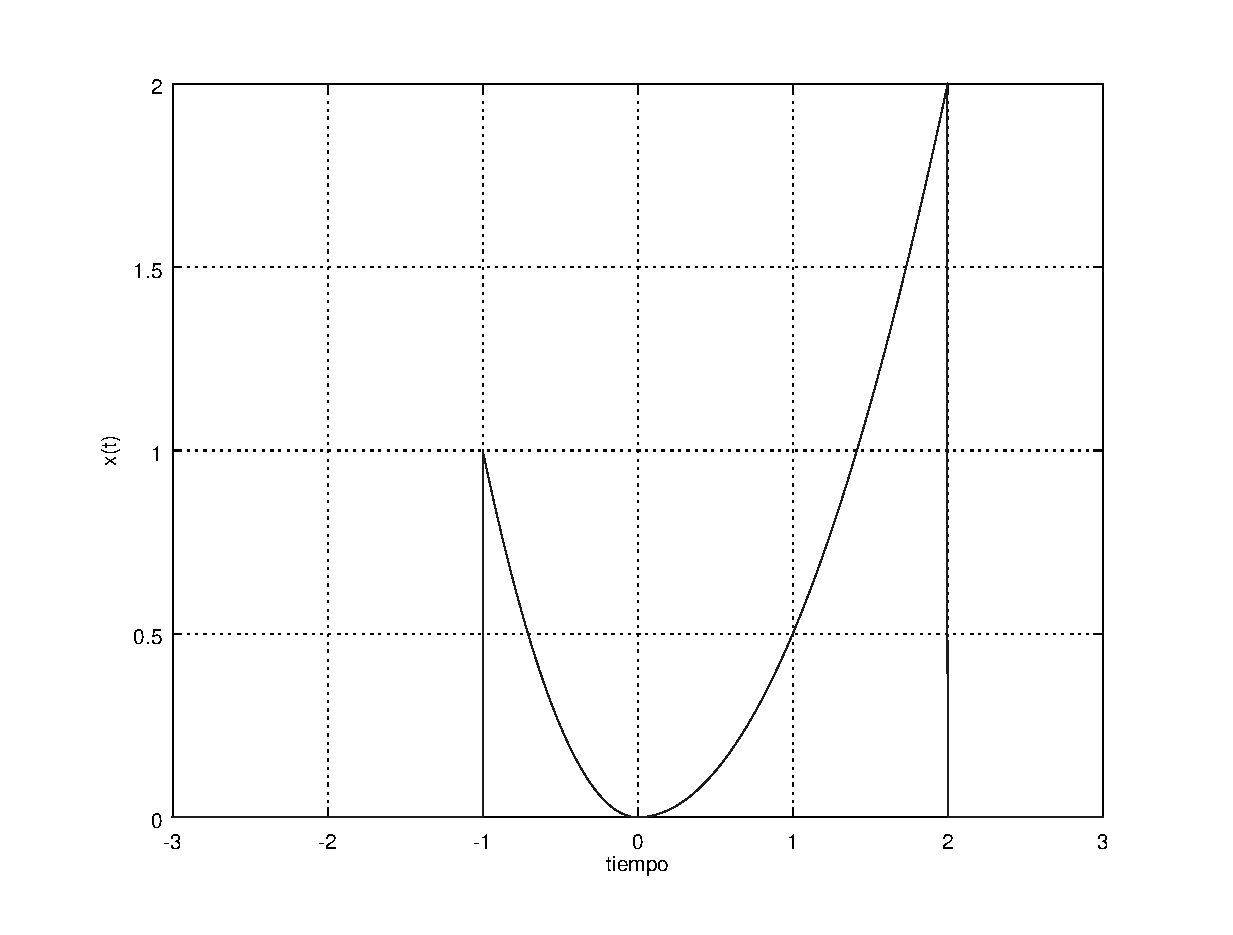
\includegraphics[width=1\linewidth]{Ejercicio1/Aproximacion2b}
        \caption{Multiplicación de ambas señales}
        \label{fig:Aprox2b}
      \end{center}
    \end{subfigure}
    
    \caption{Segunda aproximación a la señal}
    \label{fig:Aprox2}
  \end{center}
\end{figure}


Código en matlab:

\lstinputlisting{Ejercicio1/aprox2.m}

Ahora necesitamos generar el valor constante que toma la señal en sus extremos, esto lo podemos generar con la suma de otra señal $\Pi$ invertida en amplitud y desplazada hacia arriba una unidad.

\begin{figure}[H]
  \begin{center}
    
    \begin{subfigure}{0.5\textwidth}
      \begin{center}
        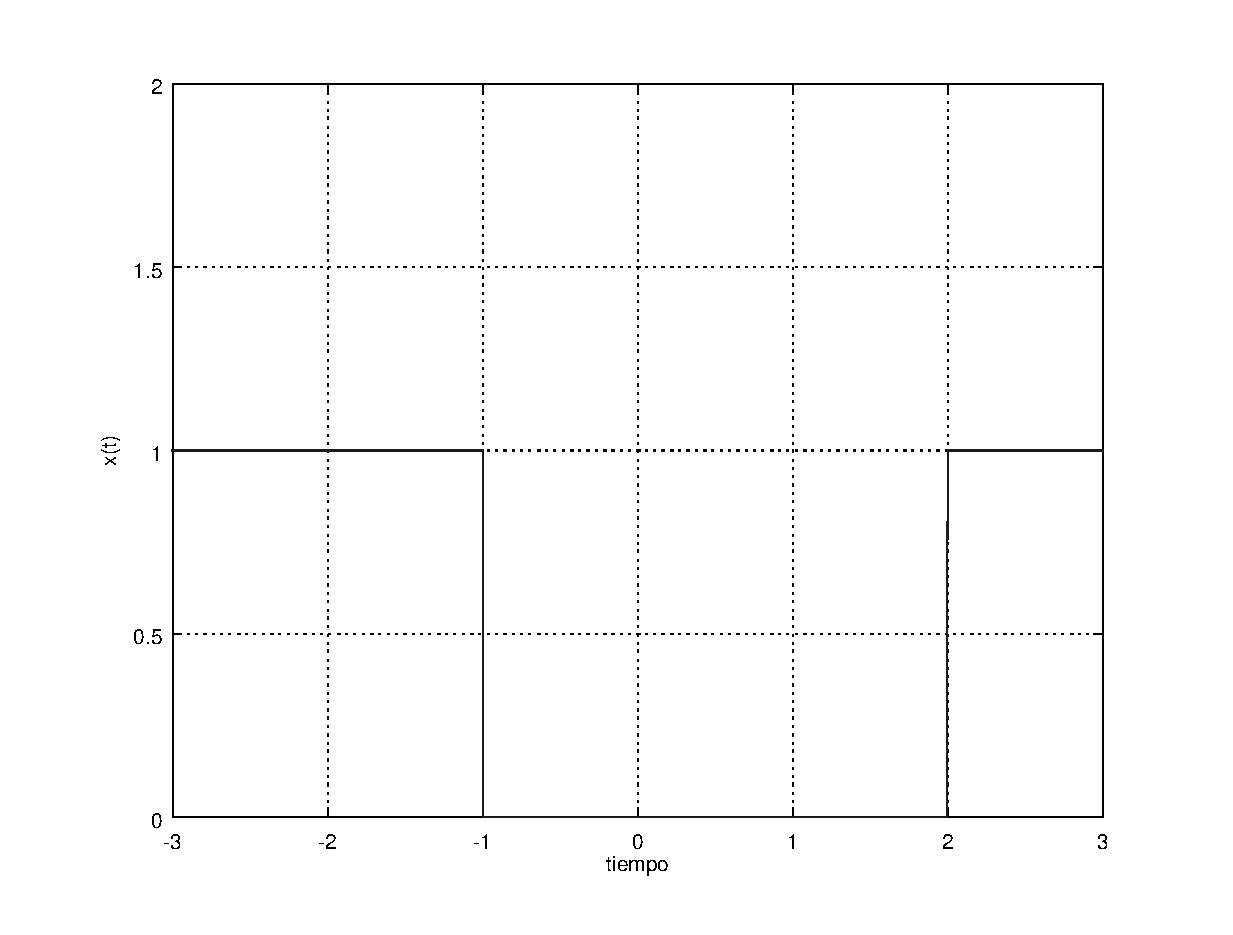
\includegraphics[width=1\linewidth]{Ejercicio1/Aproximacion3a}
        \caption{Señal $\Pi(t)$ expandida, retrasada, invertida en amplitud y trasladada una unidad hacia arriba}
        \label{fig:Aprox3a}
      \end{center}
    \end{subfigure}%    
    \begin{subfigure}{0.5\textwidth}
      \begin{center}
        \includegraphics[width=1\linewidth]{Ejercicio1/Aproximacion3b}
        \caption{Suma de ambas señales}
        \label{fig:Aprox3b}
      \end{center}
    \end{subfigure}
    
    \caption{Tercera aproximación a la señal}
    \label{fig:Aprox3}
  \end{center}
\end{figure}

Así la señal de la \texttt{figura 1.4b} es la señal expresada como funciones singulares.

\[ x(t) = \left[2u_{-3}\left(t\right)+u_{-3}\left(t\right)\right]\times\Pi\left(\frac{t-\frac{1}{2}}3\right)-\left(\Pi\left(\frac{t-\frac{1}{2}}3\right)-1\right) \] 

Código en matlab:

\begin{lstlisting}
function x = x1(t)
 x = ( ( 2*pu(-t) + pu(t) ) .* rect( (t.-0.5) ./ 3 ) ) .- ( rect( (t.-0.5) ./ 3 ) .- 1);
         
t = -15 : 0.005 : 15;
plot(t,x1(t));
axis([-3,3,0,2]);
grid();
xlabel("tiempo");
ylabel("x(t)"); 
\end{lstlisting}



\section{Ejercicio 2}
Si $x\left(t\right)$ es la que obtuvo en el Ejercicio 1, obtenga las siguientes señales:

\begin{enumerate}
  \item $x\left(\frac{t}{4}\right)$\\
  \newline Para esta gráfica la señal sufre una transformación en el tiempo, como el valor del coeficiente $\alpha$ de $t$ es igual a $\frac{1}{4}$, la señal se verá expandida en un factor inverso, es decir, la veremos cuatro veces más ancha. Esto se notará más en los limites de la parábola, los cuales irán de -4 a 8. Las funciones siempre van a tener su valor mínimo en 0, para cualquier transformación en el tiempo, además, durante la transformación la función $\Pi(t)$ sigue cortando en el mismo rango a las parábolas, por lo que la amplitud no se ve modificada.

    \begin{figure}[H]
      \begin{center}
        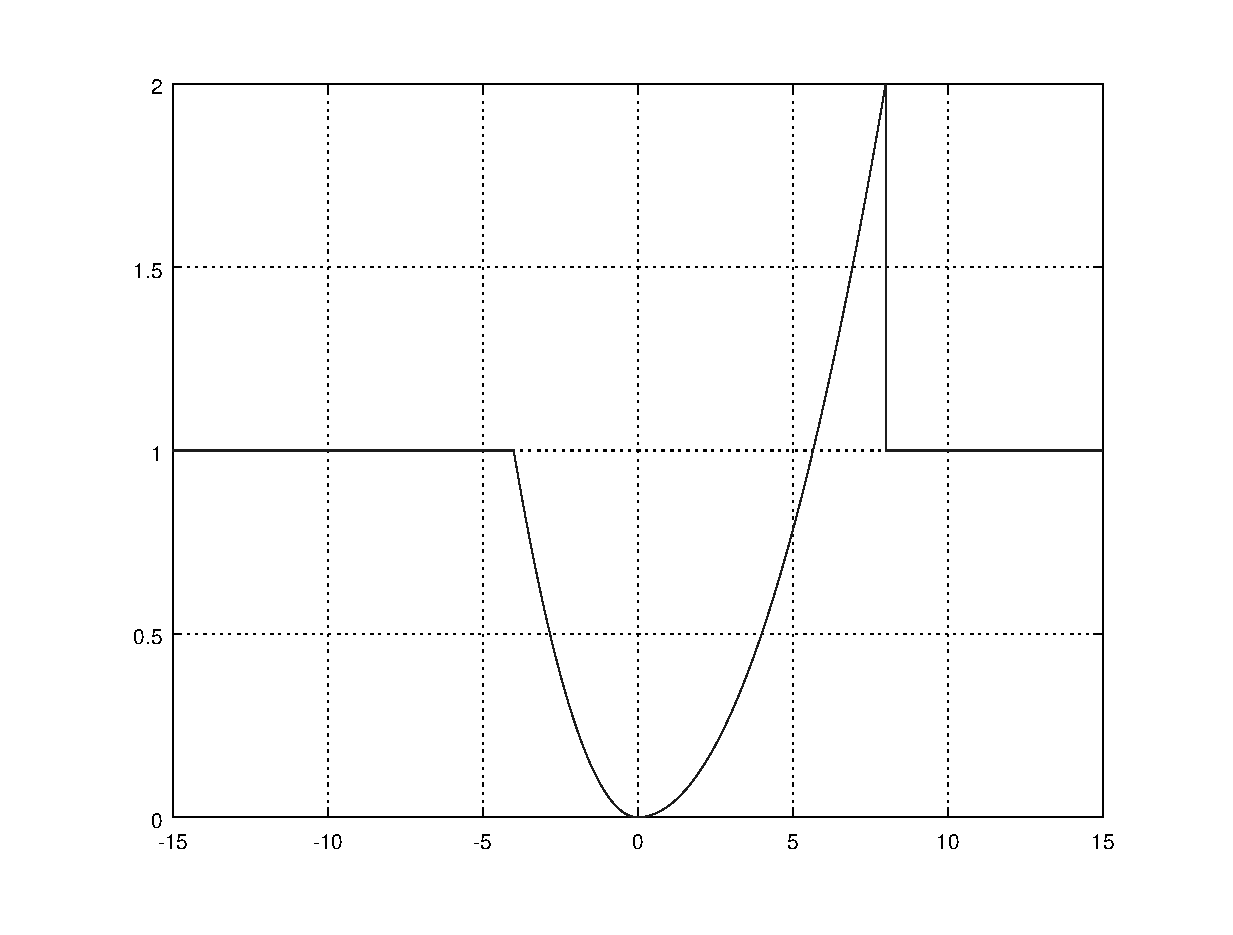
\includegraphics[width=0.5\textwidth]{Ejercicio2/IncisoA}
        \caption{Señal expandida 4 veces}
        \label{fig:IncisoA}
      \end{center}
    \end{figure}
    
Código en Matlab:
    \lstinputlisting{Ejercicio2/incisoa.m}

  \item $x\left(2t-1\right)$\\
    \newline Para nueva señal, la señal original es contraída 2 veces su ancho original y adelantada en $\frac{1}{2}$ unidad. Esto lo podemos ver mejor si reescribimos la función anterior como $x\left(2\left(t-\frac{1}{2}\right)\right)$ De forma análoga al inciso anterior, la amplitud no se modifica.

    \begin{figure}[H]
      \begin{center}
        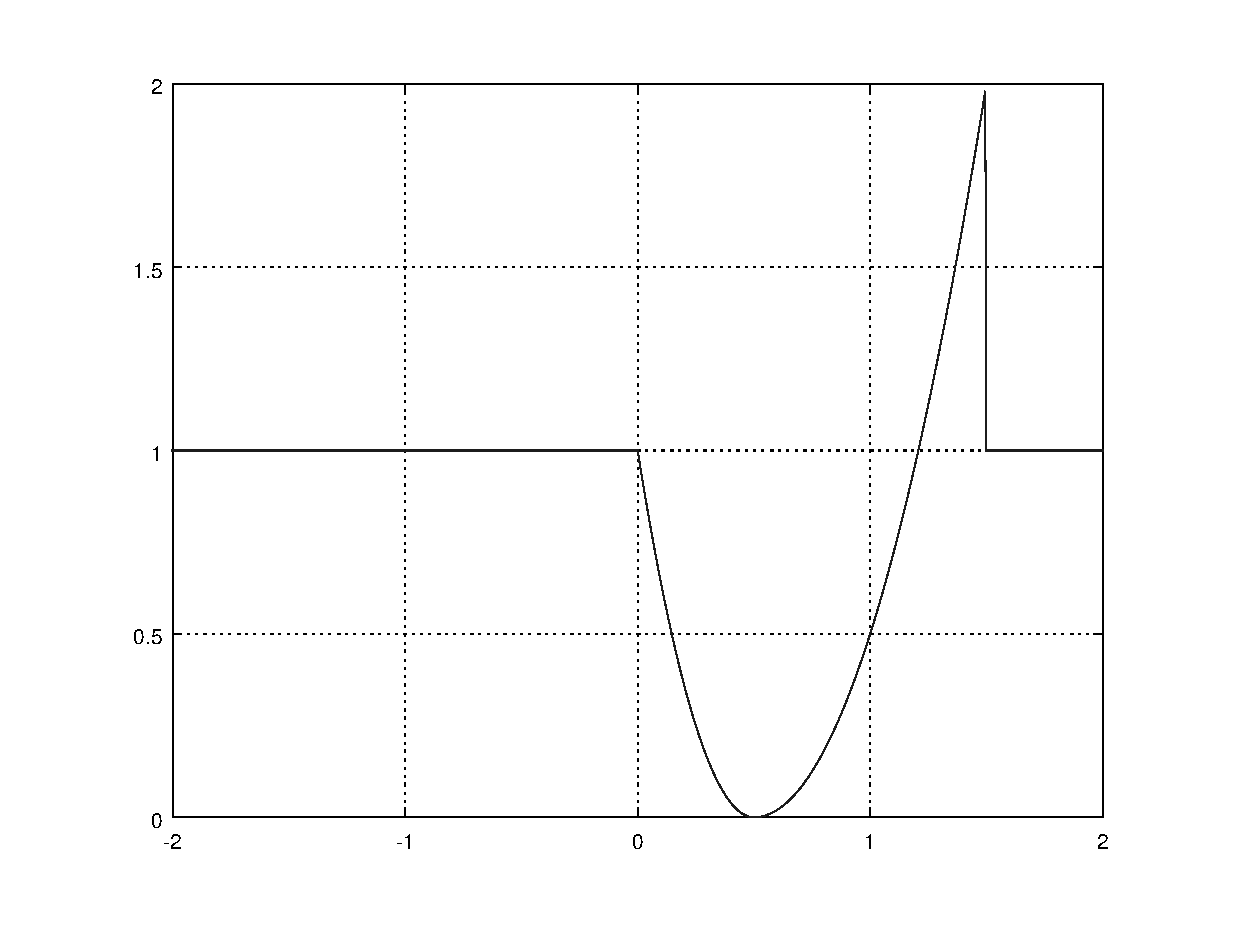
\includegraphics[width=0.5\textwidth]{Ejercicio2/IncisoB}
        \caption{Señal contraída 2 veces}
        \label{fig:IncisoB}
      \end{center}
    \end{figure}
    
Código en Matlab:
    \lstinputlisting{Ejercicio2/incisob.m}
    
  \item $x\left(-\frac{t}{4}-1\right)$\\
  \newline Si reescribimos esta señal como $x\left(-\frac{\left(t+4\right)}{4}\right)$ nos es más fácil ver que es una la señal retrasada 4 unidades, expandida 4 veces y luego invertida en el tiempo. Transformar la señal en este orden es equivalente a primero expandir la señal 4 veces y luego adelantarla 4 unidades. Nuevamente la amplitud no se ve afectada.

    \begin{figure}[H]
      \begin{center}
        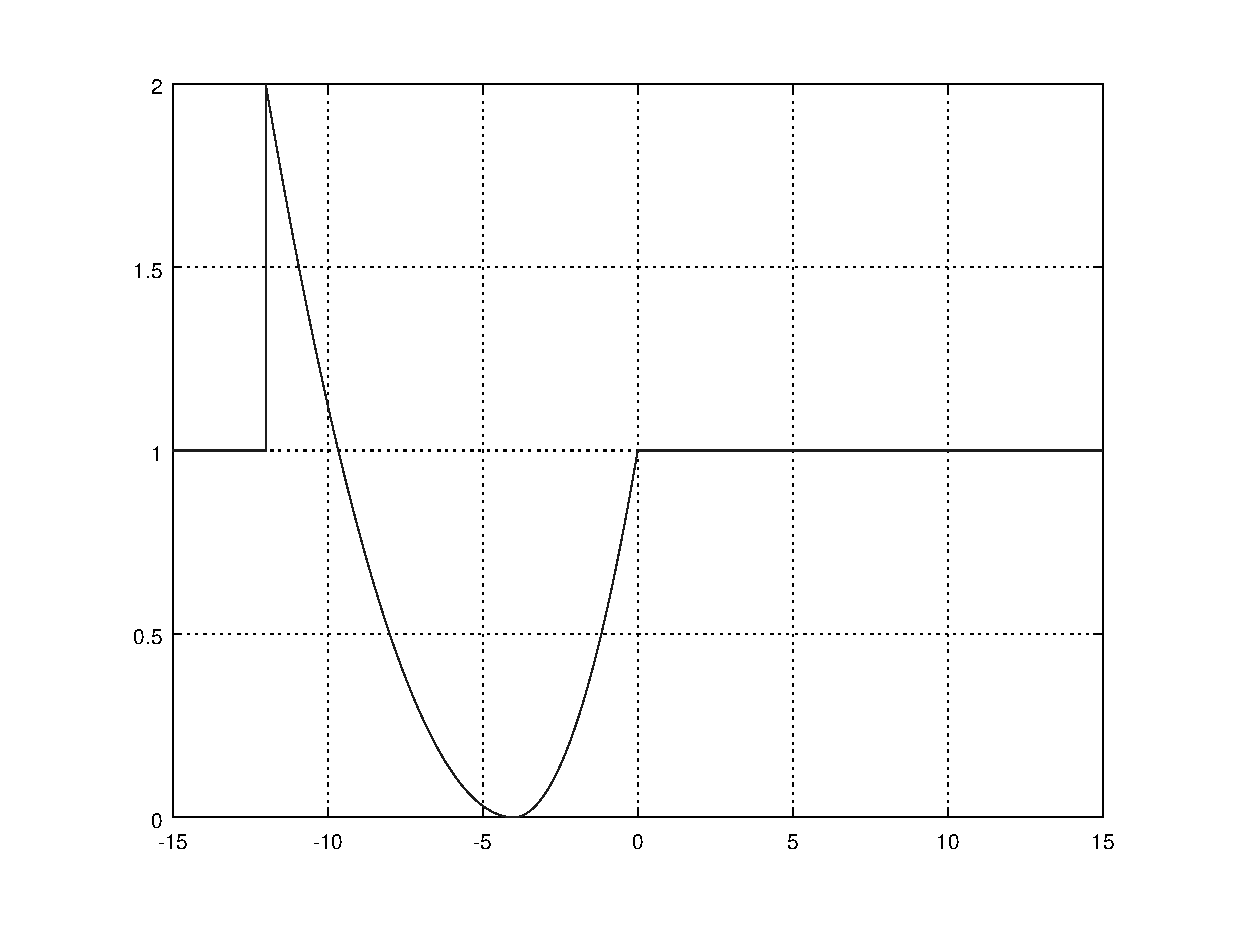
\includegraphics[width=0.5\textwidth]{Ejercicio2/IncisoC}
        \caption{Señal expandida 4 veces, invertida en el tiempo y retrasada 4 unidades}
        \label{fig:IncisoC}
      \end{center}
    \end{figure}
    
Código en Matlab:
    \lstinputlisting{Ejercicio2/incisoc.m}
    \newpage

  \item x(t/4+1/4)\\
  \newline Nuevamente reescribamos la señal para ver de forma más clara el comportamiento que presenta: $x\left(\frac{-\left(t+1\right)}{4}\right)$. En esta nueva expresión podemos ver que la señal es retrasada 1 unidad y luego expandida 4 unidades. De nuevo, la amplitud original se conserva.
    \begin{figure}[H]
      \begin{center}
        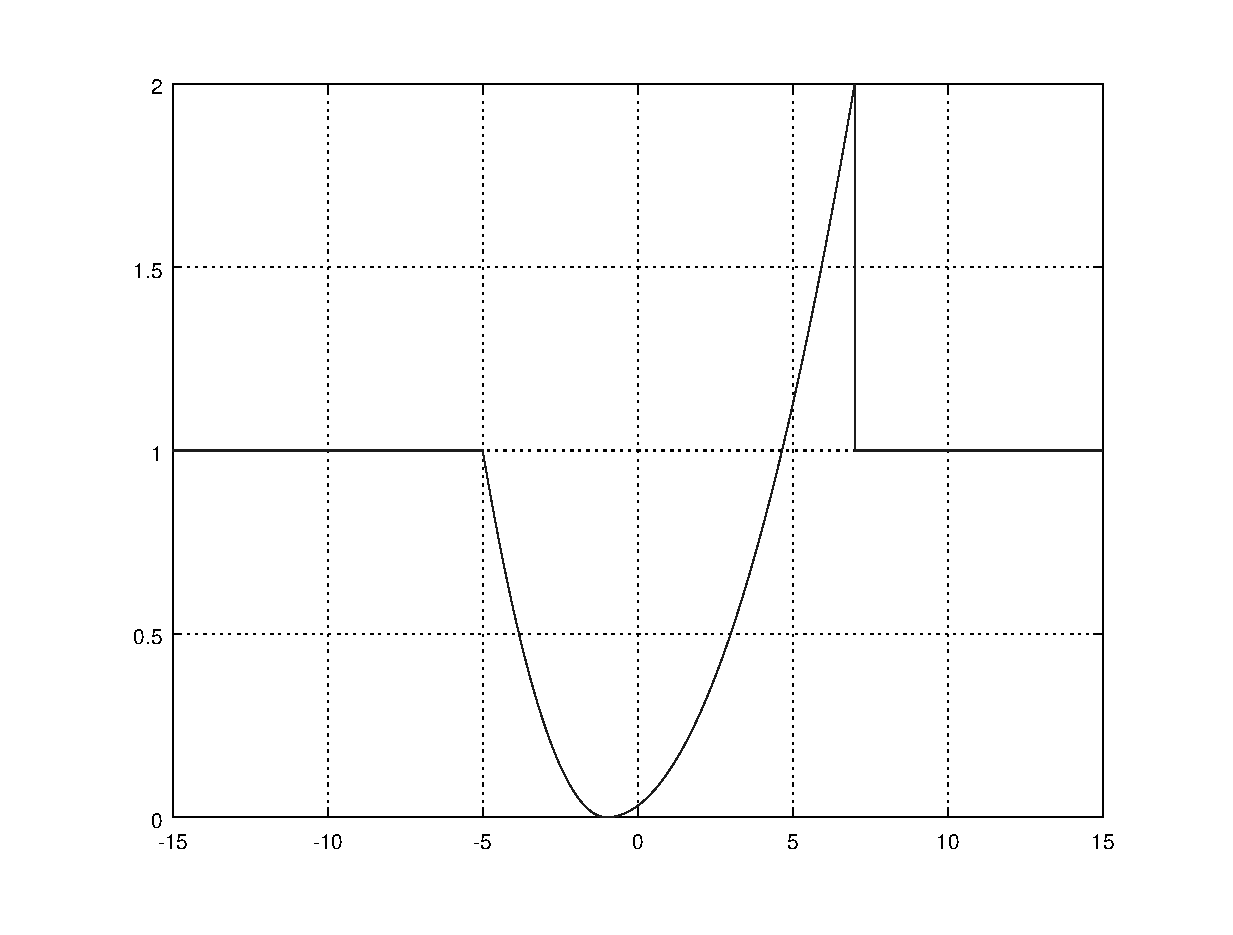
\includegraphics[width=0.5\textwidth]{Ejercicio2/IncisoD}
        \caption{Señal expandida 4 veces y retrasada 1 unidad}
        \label{fig:IncisoD}
      \end{center}
    \end{figure}
    
Código en Matlab:
    \lstinputlisting{Ejercicio2/incisod.m}
    
\end{enumerate}

\section{Ejercicio 4}
Determine si los siguientes sistemas de tiempo continuo son o no lineales, variantes en el tiempo, causales, con memoria y estables. Justifique su respuesta.
\begin{enumerate}
  \item  \[ y\left[n\right]\;=\;\left\{\begin{array}{lc}
                                     1&n\geq0 \\
                                     0&n<0 \\ 
                                   \end{array}\right.\qquad Para\;toda\;x\left[n\right]
\]
Este no es el modelo de un sistema ya que no relaciona la entrada con la salida.
  \item
    \begin{equation*}
y(t)=sen(x(t+1))
    \end{equation*}
* Lineal o no lineal

   x1(t) = y1(t)= sen (x1(t+1))\\
   x2(t) = y2(t)= sen (x2(t+1))\\
   x3(t) = x1(t)+x2(t) = y3(t)=sen(x3(t+1))\\
                         y3(t)=sen(x1(t+1)+x2(t+1))

 NO LINEAL

* Variante o invariante en el tiempo

  y(t-t0)=sen(x(t-t0+1)) ... A esto se debe llegar\\
  Proponer: x1(t)=x(t-t0) --- y1(t)=sen(x1(t+1))\\
  y1(t)=sen(x(t+1-t0))

  INVARIANTE EN EL TIEMPO

* Causalidad

y(0)=sen(x(1))\\
y(-1)=sen(x(0))\\
y(1)=sen(x(2))

NO CAUSAL O ANTICIPATIVO, porque depende de valores futuros.

* Memoria

CON MEMORIA, por que depende de valores futuros.

* Estabilidad

ESTABLE, ya que al probar con una señal como el escalón, la entrada y la salida es acotada.

\end{enumerate}

\section{Ejercicio 5}

Evalúe las siguientes integrales:
\[
y(t)=\int_{-\infty }^{\infty }[3\delta (t)+e^{-(t-1)}\delta (t)+cos(2\pi t)\dot{\delta} (t)+e^{-t}\ddot{\delta }(t) ]dt
\]

\[
y(t)=\int_{0}^{\infty }e^{-(t-1)}\delta (t+10)dt
\]

Para la primera ecuación tenemos que gracias a la propiedad de linealidad podemos realizar esta descomposición:

\[
y(t)=3\int_{-\infty }^{\infty }\delta (t)dt+\int_{-\infty }^{\infty }e^{-(t-1)}\delta (t)dt+\int_{-\infty }^{\infty }cos(2\pi t)\dot{\delta (t)}dt+\int_{-\infty }^{\infty }e^{-t}\ddot{\delta}(t)dt
\]\\
Sabiendo que la transformada de Laplace de delta de Dirac es:
\[
L\left \{ \delta \left ( t \right ) \right \}=1
\]\\
Y que:
\[
L\left \{ f(t)\delta (t-a) \right \}=\int_{0 }^{\infty }e^{-st}f(t)\delta (t-a)dt=e^{-as}f(a)
\]\\
Basándonos en esos conceptos ya nos es posible operar\\
Utilizando la transformada de Laplace
\[
3L\left \{ \delta (t) \right \}=3\ast 1=3
\]\\
Aplicando la transformada al otro termino quedaría:
\[
L\left \{ e^{-(t-1)}\delta (t) \right \}
\]\\
Ayudándonos de la ecuación numero 5 tenemos que a=0 por lo tanto:\\
\[
e^{-as}\cdot f(a)=e^{-0s}\cdot e^{-(0-1)}=e^{o}\cdot e^{1}=1\cdot e=e
\]\\

Pasando al otro termino de la ecuación tendríamos:
\[
L\left \{ cos(2\pi t)\dot{\delta }(t) \right \}
\]\\
La transformada de la derivada de la función impulso va a ser cero:
\[
L\left \{ \dot{\delta }(t) \right \}=0
\]\\
Aplicando la ecuación numero 5 obtendremos:
\[
0\cdot cos(2\pi (0))=0\cdot 1=0
\]\\
Para nuestro ultimo termino.\\
La tranformada de la segunda derivada de la función impulso es cero:
\[
L\left \{ \ddot{\delta }(t) \right \}=0
\]\\
Evaluando con base a la ecuación 5 tendremos:
\[
0\cdot e^{-0}=0\cdot 1=0
\]\\
Por ultimo sumamos nuestros resultados y nos quedaría:
\[
3+e+0+0=3+e
\]\\
Finalmente nuestro resultado es:
\[
\underline{3+e}
\]\\

Para nuestra otra función integral tendremos que a=10:
\[
\left [ e^{-10}\cdot e^{-(10-1)} \right ]=e^{-10}\cdot e^{-10}\approx 0.00000000206= 0
\]\\
Finalmente este es nuestro resultado:
\[
\underline{0}
\]\\







\section{Ejercicio 6}
Grafique las siguientes señales:
\begin{equation*}
x(t)=rect(2t-0.5)
\end{equation*}

\begin{figure}[H]
\centering
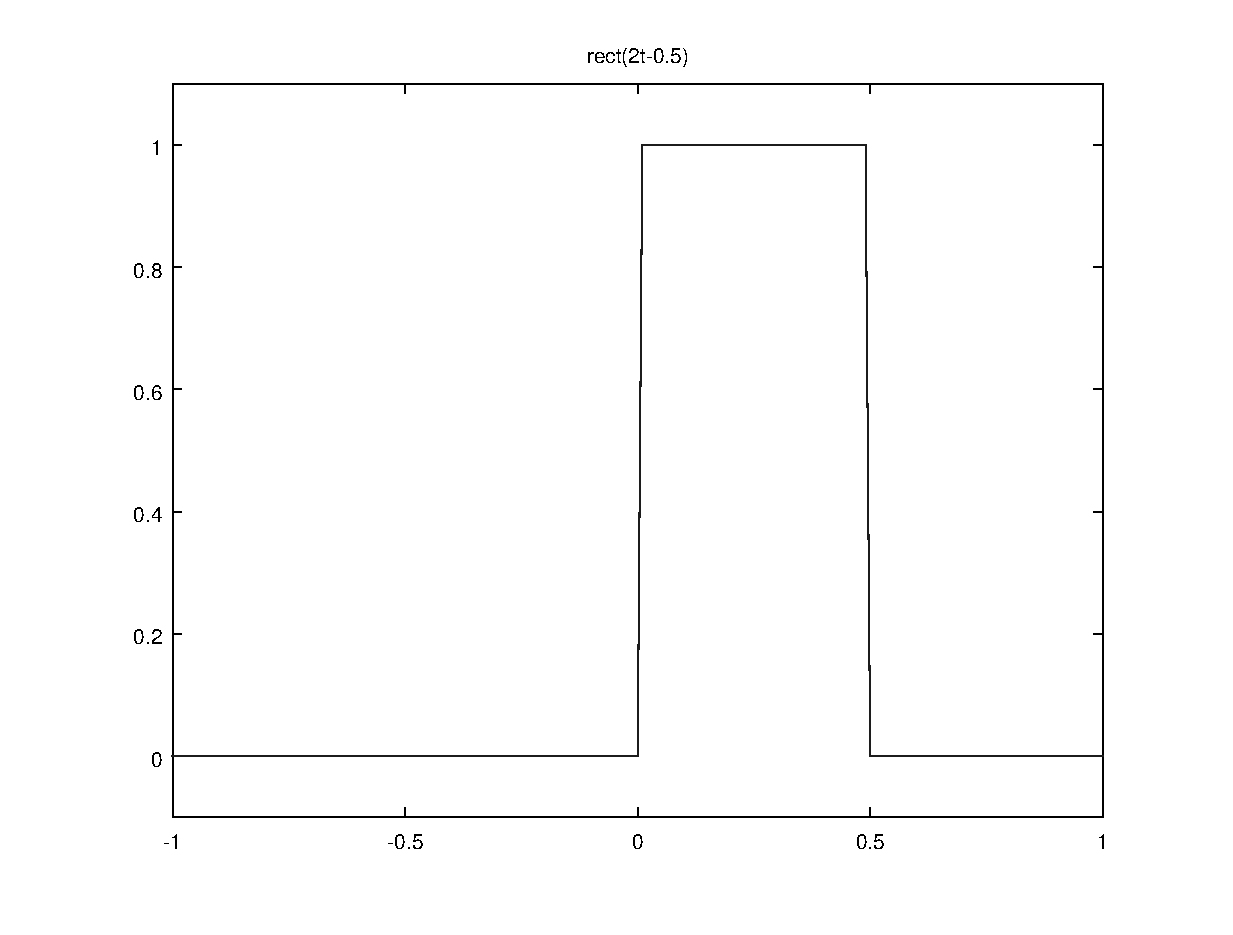
\includegraphics[width=0.6\textwidth]{rectA}
\caption{rect(2t - 0.5)}
\label{fig:rectA}
\end{figure}

\begin{equation*}
x(t)=rect((t-1)/2)+(t-1))
\end{equation*}

\begin{figure}[H]
\centering
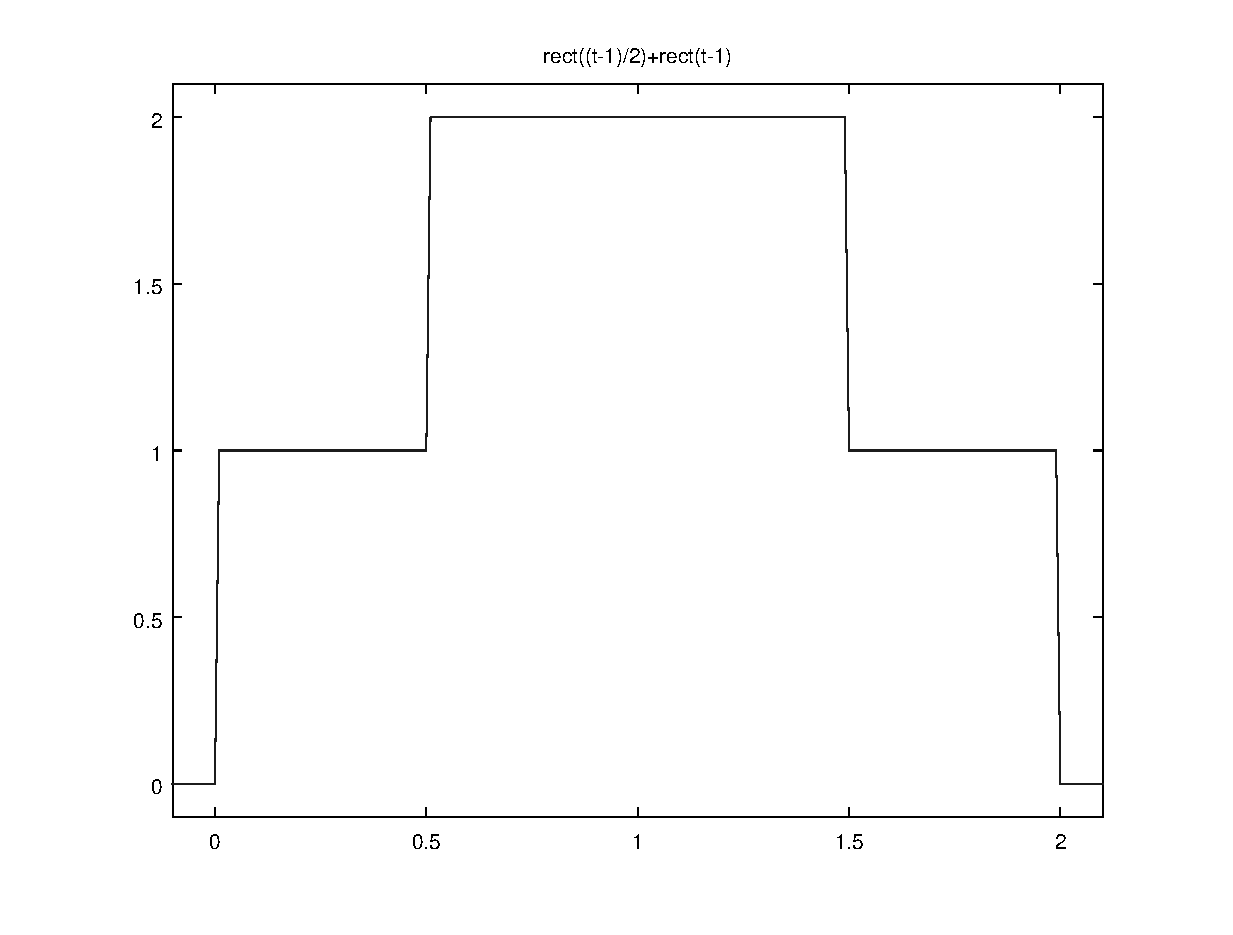
\includegraphics[width=0.6\textwidth]{rectB}
\caption{rect((t-1)/2)+(t-1)}
\label{fig:rectB}
\end{figure}








\section{Ejercicio 8}
Capture al menos dos señales físicas reales y preséntelas en una  gráfica e identifique el tipo de señal en algún segmento de la misma.\\

\begin{itemize}
\item La primera señal es un silbido humano.\\
Código de Matlab:\\
\begin{lstlisting}[frame=single]
>> [y,Fs] = audioread('Silb.wav');
>> sound(y,Fs);
>> figure(2);
>> plot(y);
\end{lstlisting}

\begin{figure}[htb]
\centering
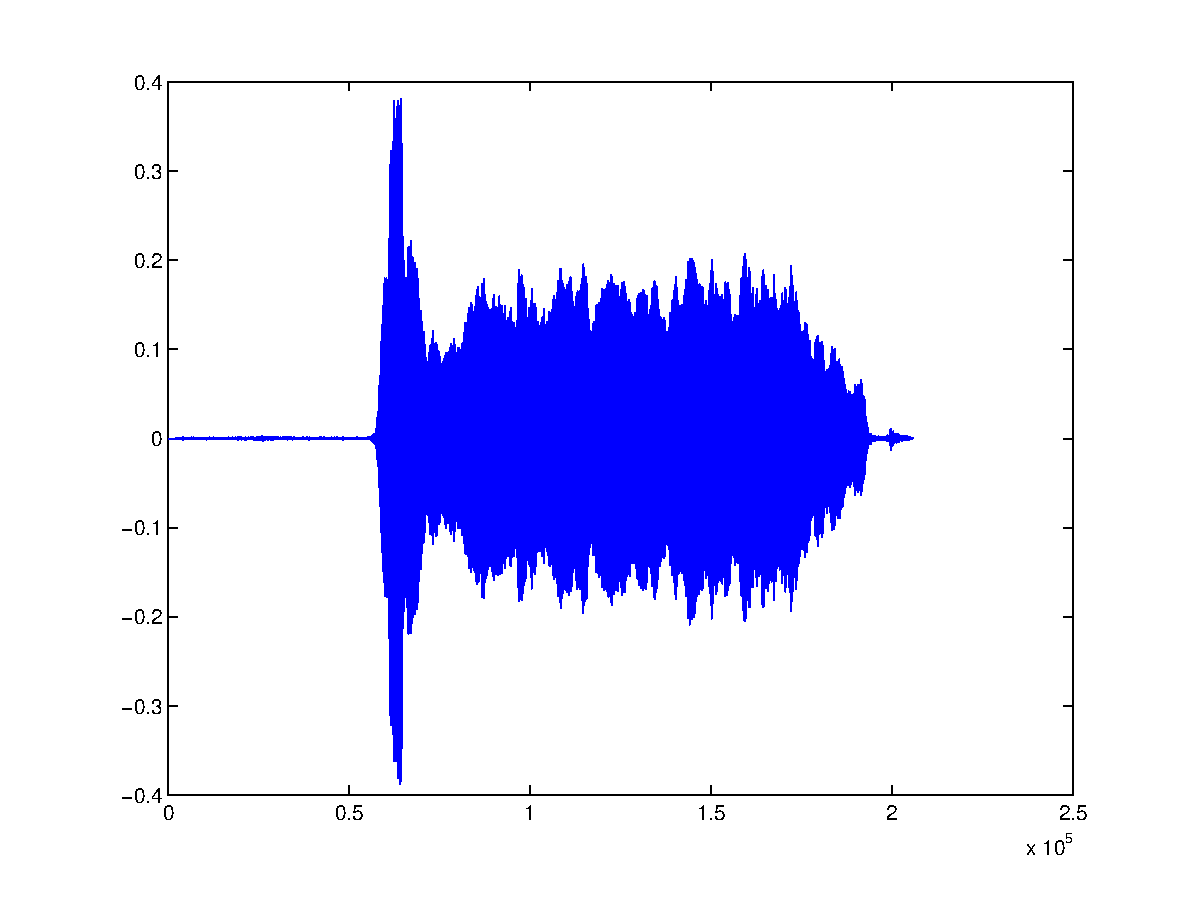
\includegraphics[width=0.6\textwidth]{SilbGraphic}
\caption{Silbido humano}
\label{fig:SilbGraphic}
\end{figure}

Esta es una señal de tiempo continuo por que la señal puede tomar cualquier valor en cualquier instante de tiempo. \\
Es una señal aperiódica, ya que no se repite en intervalos regulares \\
Es una señal aleatoria, ya que no se puede predecir mediante una función matemática.\\
Notamos en la gráfica que la señal el totalmente impredecible, ya que siempre parece tomar diferentes valores de frecuencia.

\item La segunda señal corresponde al sonido de las cuerdas de una guitarra acústica.\\
Código de Matlab:\\
\begin{lstlisting}[frame=single]
>> [y,Fs] = audioread('Guitar.wav');
>> sound(y,Fs);
>> figure(1);
>> plot(y);
\end{lstlisting}

\begin{figure}[H]
\centering
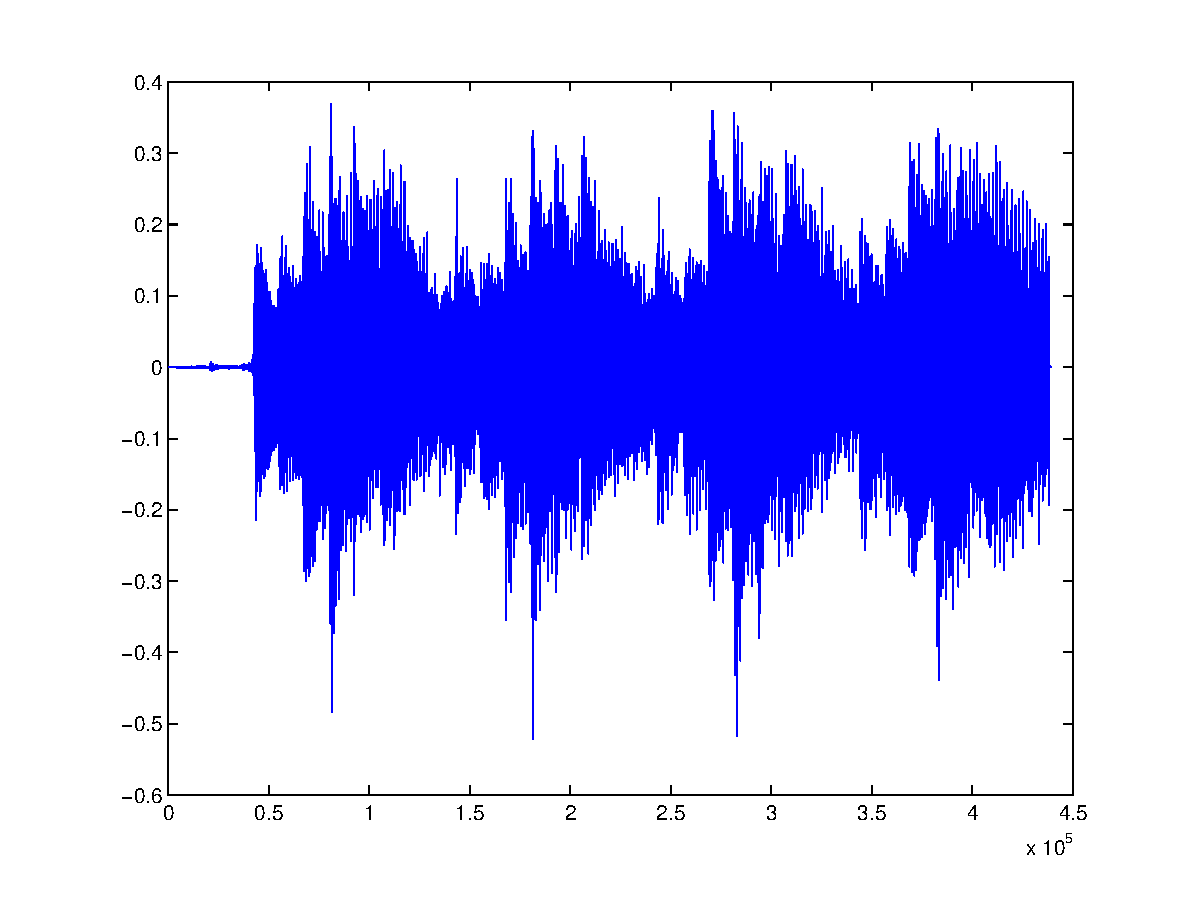
\includegraphics[width=0.6\textwidth]{GuitarGraphic}
\caption{Sonido de las cuerdas de una guitarra acústica}
\label{fig:GuitarGraphic}
\end{figure}

Esta es una señal de tiempo continuo por que la señal puede tomar cualquier valor en cualquier instante de tiempo. \\
Es una señal aperiódica, ya que no se repite en intervalos regulares \\
Es una señal aleatoria, ya que no se puede predecir mediante una función matemática.\\
NOTA: Se trató de que el rasgeo de las cuerdas de la guitarra sean igual en tiempo e intensidad, resultó un poco difícil, el mejor de los casos qes que hubiera salido igual la gráfica en intervalos regulares, para que la señal sea periódica y determinística.

\end{itemize}

\section{Ejercicio 9}

Conexión de sistemas en serie o cascada\\
\[
S_{1}: y_{1}\left [ n \right ]=x_{1}\left [ n \right ]+2x_{1}\left [ n-1 \right ]
\]
\[
S_{2}: y_{2}\left [ n \right ]=x_{2}\left [ n+2 \right ]+3x_{2}\left [ n \right ]
\]\\

S:\\
\[
x_{2}\left [ n \right ]=y_{1}\left [ n \right ]=x_{1}\left [ n \right ]+2x_{1}\left [ n-1 \right ]
\]
\[
x_{2}\left [ n+2 \right ]=x_{1}\left [ n+2 \right ]+2x_{1}\left [ n+2-1 \right ]
\]
\[
3x_{2}\left [ n \right ]=3x_{1}\left [ n \right ]+(3)2x_{1}\left [ n-1 \right ]
\]\\

\[
y\left [ n \right ]=y_{2}\left [ n \right ]=x_{1}\left [ n+2 \right ]+2x_{1}\left [ n+1 \right ]+3x_{1}\left [ n \right ]+6x_{1}\left [ n-1 \right ]
\]
\[
y\left [ n \right ]=6x_{1}\left [ n-1 \right ]+3x_{1}\left [ n \right ]+2x_{1}\left [ n+1 \right ]+x_{1}\left [ n+2 \right ]
\]\\

Ahora sacaremos su sistema invertido\\
\[
x_{1}\left [ n \right ]=y_{2}\left [ n \right ]=x_{2}\left [ n+2 \right ]+3x_{2}\left [ n \right ]
\]
\[
x_{1}\left [ n \right ]=x_{2}\left [ n+2 \right ]+3x_{2}\left [ n \right ]
\]
\[
2x_{1}\left [ n-1 \right ]=2x_{2}\left [ n-1+2 \right ]+(2)3x_{2}\left [ n-1 \right ]
\]\\

\[
x\left [ n \right ]=x_{2}\left [ n \right ]=x_{2}\left [ n+2 \right ]+3x_{2}\left [ n \right ]+2x_{2}\left [ n+1 \right ]+6x_{2}\left [ n-1 \right ]
\]
\[
x\left [ n \right ]=6x_{2}\left [ n-1 \right ]+3x_{2}\left [ n \right ]+2x_{2}\left [ n+1 \right ]+x_{2}\left [ n+2 \right ]
\]\\

Vemos que el sistema normal e invertido da el mismo resultado.

\section{Ejercicio 10}

Conexión de sistemas en serie o cascada\\

\[
S_{1}: y_{1}\left [ n \right ]=nx_{1}\left [ n \right ]
\]
\[
S_{2}: y_{2}\left [ n \right ]=x_{2}\left [ -n-1 \right ]
\]\\

S:\\

\[
x_{2}\left [ n \right ]=y_{1}\left [ n \right ]=nx_{1}\left [ n \right ]
\]
\[
x_{2}\left [ -n-1 \right ]=nx_{1}\left [ -n-1 \right ]
\]\\

\[
y\left [ n \right ]=y_{2}\left [ n \right ]=nx_{1}\left [ -n-1 \right ]
\]
\[
y\left [ n \right ]=nx_{1}\left [ -n-1 \right ]
\]\\

Ahora sacaremos su sistema invertido\\
\[
x_{1}\left [ n \right ]=y_{2}\left [ n \right ]=x_{2}\left [ -n-1 \right ]
\]
\[
nx_{1}\left [ n \right ]=nx_{2}\left [ -n-1 \right ]
\]
\[
x\left [ n \right ]=nx_{2}\left [ -n-1 \right ]
\]\\

Vemos que el sistema normal e invertido da el mismo resultado.










\end{document}
